\pagebreak
\section{Digital Analog Converter (DAC) e Comparatore}
\label{DAC}
Il DAC e il Comparatore, anche se 2 periferiche diverse, sono trattate insieme in quanto sono usate come trigger: il DAC per generare un segnale analogico e il comparatore per confrontare il segnale generato con un segnale di riferimento, così facendo si può avere un meccanismo di Trigger molto preciso e veloce.\\

\subsection{Funzionamento DAC}

Il DAC del microcontrollore è una periferica a 12 bit che permette di generare un segnale analogico a partire da un segnale digitale.\\ 
Una grande problematica del DAC è la gestione dell'errore. Infatti, se si vuole generare un segnale analogico ad un determinato voltaggio a partire da un numero binario, a prescindere dalla struttura, ci sarà sempre un errore dovuto alla lunghezza del numero binario. A questo errore si aggiungono tutti gli errori strumentali delle componenti del DAC.\\

Per questo motivo, la struttura del DAC è stata progettata in modo da minimizzare l'errore. Questa struttura è detta \textit{R-2R} e consiste in una rete di resistenze dal valore di $R$ e $2R$.

\begin{figure}[h]
    \centering
    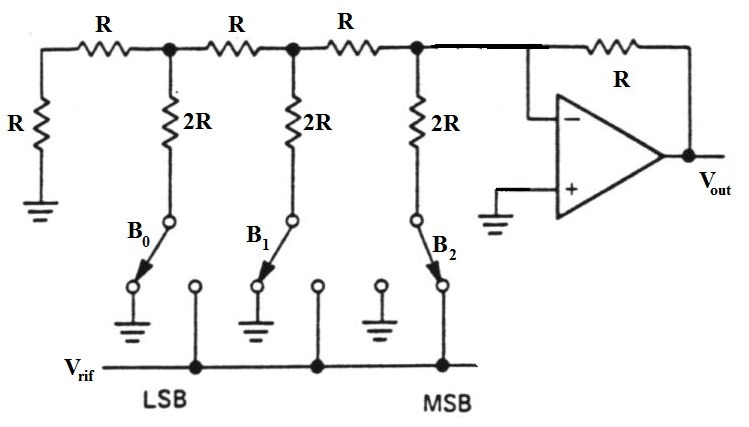
\includegraphics[width=0.7\linewidth]{microcontrollore/assets/DACr2r.jpg}
    \caption{Struttura interna del DAC}
    \label{fig:DAC}
\end{figure}

La struttura è molto semplice: ogni switch corrisponde ad un transistor a cui viene dato il valore del bit in voltaggio: se il bit è 1, il circuito si chiude e il voltaggio in uscita è $V_{ref}$, se il bit è 0, il circuito si apre e il voltaggio in uscita è 0. La configurazione delle Resistenze permette di dimezzare il voltaggio in uscita ad ogni iterazione dello schema. E, dato che alla fine c'è un amplificatore operazionale, il voltaggio in uscita sarà la somma dei voltaggi generati da ogni bit, moltiplicato per un fattore dell'Amplificatore.\\

Così facendo, usando solo 2 tipi di resistenza, un amplificatore operazionale e dei transistor come interruttori, siamo in grado di creare un segnale analogico.\\
\pagebreak
\subsection{Funzionamento Comparatore}
Il Comparatore non è altro che un amplificatore operazionale con un'uscita che non può essere Negativa. Questo significa che, se il voltaggio in ingresso è maggiore di un voltaggio di riferimento, l'uscita sarà alta, altrimenti sarà bassa.\\

\begin{wrapfigure}{r}{0.4\linewidth}
    \centering
    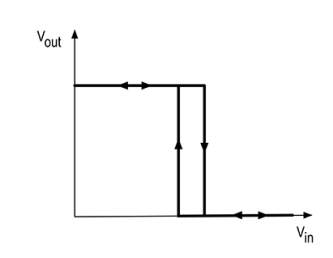
\includegraphics[width=\linewidth]{microcontrollore/assets/Hysteresis.png}
    \caption{Grafico Voltaggio Amplificatore con Isteresi}
    \label{fig:Comparatore}
\end{wrapfigure}

Se si considera un comparatore ideale, questo soffrirà di instabilità nel caso in cui il voltaggio in input sia vicino al voltaggio di riferimento. Per evitare questo problema, si aggiunge l'isteresi al comparatore.\\
L'isteresi si ottiene mettendo il comparatore in retroazione positiva, così facendo, il voltaggio di salita si discosta dal voltaggio di discesa, evitando quindi il problema di instabilità del comparatore.\\

Questa particolare caratteristica del comparatore ci permetterà di usare il comparatore non solo come singolo trigger ma come doppio trigger.\\

\subsection{Programmazione}
La programmazione del DAC e del Comparatore si fa quasi totalmente da STM32CubeMX. La configurazione consiste nel collegare il DAC al comparatore, selezionre il valore di isteresi del Comparatore. Una volta configurato, nel codice basta aggiungere la funzione che permette di attivare il DAC e il Comparatore.\\

\begin{minted}[bgcolor=coding , linenos]{C}
    COMP2->CFGR |= COMP_CFGRx_EN; // Attiva il Comparatore
    DAC1 -> DHR12R1 = 1000;	// soglia di trigger
	DAC1 -> SWTRIGR |= DAC_SWTRIGR_SWTRIG1; // Abilita il software trigger
	DAC1 -> CR |= DAC_CR_EN1; // Attiva il DAC
\end{minted}

E, per andare a controllare lo stato del comparatore, si può usare la funzione:

\begin{minted}[bgcolor=coding , linenos]{C}
if( COMP12 -> SR & COMP_SR_C2VAL){ // Se il comparatore è attivo
    //Fai qualcosa
}
\end{minted}